\documentclass{article}

\usepackage[dblblindworkshop]{neurips_2026}
\usepackage[utf8]{inputenc}
\usepackage[T1]{fontenc}
\usepackage{hyperref}
\usepackage{url}
\usepackage{booktabs}
\usepackage{amsmath}
\usepackage{amsfonts}
\usepackage{amssymb}
\usepackage{microtype}
\usepackage{xcolor}
\usepackage{graphicx}
\usepackage{subcaption}
\usepackage{multirow}

\title{Self Verification Through Hidden Visual Evidence in Vision Language Models}
\author{Anonymous Authors}

\begin{document}
\maketitle

\begin{abstract}
Vision language models can identify image regions that influence an answer without determining whether those regions actually justify the answer. We study this distinction using hidden state interventions. For each image question pair, we blur each cell in a $6\times6$ image grid, rank cells by the resulting hidden state change, and evaluate the selected regions using exact COCO segmentation masks and behavioral interventions. On a controlled benchmark of 100 previously unused COCO images, hidden state ranking achieves patch average precision of $0.761$ for Qwen2.5 VL 7B and $0.689$ for Qwen2.5 VL 3B, compared with $0.397$ and $0.405$ for random ranking. The top selected region intersects the annotated target in $88.5\%$ and $84.8\%$ of held out examples. Removing the top three regions reduces answer probability by $0.211$ and $0.161$ more than matched random removal, while retaining only those regions increases answer probability by $0.508$ and $0.339$ over random evidence. However, a hallucination verification score that reaches $0.747$ AUROC in a Qwen 7B discovery experiment falls to $0.558$ under frozen transfer to Qwen 3B. These results establish a localization verification gap: causal visual evidence can reveal what drives an answer without revealing whether the answer is correct.
\end{abstract}

\section{Introduction}

Large vision language models can produce the same answer for very different reasons. A model may answer yes because the queried object is visible, because a visually similar object is present, or because the scene strongly suggests the object. These cases are difficult to distinguish from the output alone, especially when the model is confident.

Visual attribution methods attempt to identify the image regions responsible for a prediction \citep{selvaraju2017gradcam,fong2017meaningful}. Yet a plausible heatmap does not by itself establish that the highlighted evidence is faithful, causal, or semantically valid \citep{adebayo2018sanity,jain2019attention,wiegreffe2019attention}. This distinction matters for hallucination detection. A region may genuinely cause a model to answer car while containing an airport service vehicle rather than a car. In that case, localization succeeds while verification fails.

We study this gap through controlled hidden state interventions. We divide an image into patches, blur each patch independently, and rank patches by the relative change in a selected hidden representation. We then evaluate two different questions:

\begin{enumerate}
    \item \textbf{Localization:} Do the selected regions overlap the annotated object and causally affect the model's answer?
    \item \textbf{Verification:} Does the strength or sufficiency of the selected evidence distinguish grounded answers from hallucinated answers?
\end{enumerate}

We evaluate Qwen2.5 VL 7B and 3B \citep{bai2025qwen25vl} on POPE \citep{li2023pope} and on a controlled COCO evidence benchmark built from images with exact instance masks \citep{lin2014coco}. The results show that hidden state perturbation transfers as a causal localization method, but its use as a general hallucination verifier does not.

Our contributions are:

\begin{itemize}
    \item A model agnostic hidden state perturbation procedure for ranking visual evidence regions.
    \item A controlled COCO evaluation of localization, necessity, and sufficiency across two model sizes.
    \item Evidence that localization is robust across models while a frozen verification score does not transfer.
    \item A qualitative failure analysis separating localized false cues, diffuse scene priors, and semantic or annotation ambiguity.
\end{itemize}

\section{Related Work}

\paragraph{Object hallucination.}
POPE introduced a polling based evaluation of object hallucination in large vision language models \citep{li2023pope}. Subsequent benchmarks and mitigation methods have examined visual illusions, free form hallucination, and visually grounded decoding \citep{guan2024hallusionbench,kaul2024throne,leng2024vcd,favero2024m3id}. These methods primarily evaluate or modify the final answer. Our focus is complementary: we test whether internal visual evidence is causally faithful and whether that faithfulness is sufficient for verification.

\paragraph{Visual explanations.}
Grad CAM and perturbation methods localize input regions related to a prediction \citep{selvaraju2017gradcam,fong2017meaningful}. Sanity checks have shown that visual appeal alone is not enough to establish faithfulness \citep{adebayo2018sanity}. Our evaluation therefore uses segmentation overlap, matched random controls, and direct necessity and sufficiency interventions.

\paragraph{Explanations versus correctness.}
Prior work has questioned whether internal importance signals should be treated as explanations \citep{jain2019attention,wiegreffe2019attention}. We extend this question to multimodal hallucinations. The central distinction in our work is between evidence that causally drives an answer and evidence that semantically justifies that answer.

\section{Method}

\subsection{Hidden visual evidence}

Let $I$ be an image, $q$ a binary object question, and $h_{\ell}(I,q)$ the hidden representation at layer $\ell$ immediately before the first answer token. We partition the image into $M=36$ grid cells. For each cell $j$, we create $I^{(j)}$ by applying Gaussian blur only inside that cell. The hidden evidence score is

\begin{equation}
 s_j = \frac{\lVert h_{\ell}(I^{(j)},q)-h_{\ell}(I,q)\rVert_2}
 {\lVert h_{\ell}(I,q)\rVert_2+\epsilon}.
\end{equation}

We use a layer at approximately $75\%$ of model depth, layer 21 for Qwen 7B and layer 27 for Qwen 3B. The top $k$ evidence set is $T_k=\operatorname{TopK}(s_1,\ldots,s_M)$ for $k\in\{1,3,5\}$.

\subsection{Localization}

For target present examples, COCO instance masks identify which patches intersect the queried object. We report patch average precision, the rank of the first target patch, top $k$ target hit, and target mask coverage. We compare hidden state ranking with:

\begin{itemize}
    \item output probability drop after blurring each patch,
    \item CLIP similarity between the target name and each patch crop \citep{radford2021clip},
    \item a center prior,
    \item random ranking,
    \item an annotation oracle.
\end{itemize}

\subsection{Necessity and sufficiency}

Localization does not establish causal influence. We therefore measure two paired intervention effects.

For necessity, we blur all patches in $T_k$ and measure the drop in yes probability. We subtract the effect of a matched random set $R_k$:

\begin{equation}
N(k)=\left[p_{\mathrm{yes}}(I,q)-p_{\mathrm{yes}}(I\setminus T_k,q)\right]
-\left[p_{\mathrm{yes}}(I,q)-p_{\mathrm{yes}}(I\setminus R_k,q)\right].
\end{equation}

For sufficiency, we keep the selected patches visible and blur the rest of the image:

\begin{equation}
S(k)=p_{\mathrm{yes}}(I[T_k],q)-p_{\mathrm{yes}}(I[R_k],q).
\end{equation}

Positive values indicate that hidden evidence is more behaviorally important than random evidence.

\subsection{Verification}

The verification task compares grounded yes answers with hallucinated yes answers, so both classes share the same clean output. In the Qwen 7B discovery experiment, mask type, $k$, and score were selected using validation data. The selected score used top three evidence sufficiency. We then froze the method and direction for transfer to Qwen 3B. Only a decision threshold was selected on the new validation split.

\section{Experimental Setup}

\paragraph{Models.}
We evaluate Qwen2.5 VL 7B Instruct and Qwen2.5 VL 3B Instruct \citep{bai2025qwen25vl}. Generation is deterministic and restricted to yes or no. The yes probability is normalized over first token probabilities assigned to yes and no.

\paragraph{POPE verification sets.}
We construct confidence matched, image disjoint pairs of grounded yes and hallucinated yes answers across POPE adversarial, popular, and random categories. The Qwen 7B discovery evaluation contains 40 examples. The frozen Qwen 3B transfer evaluation contains 72 examples, with 12 matched pairs per POPE category.

\paragraph{Controlled COCO evidence benchmark.}
We sample 100 previously unused POPE images whose queried COCO object has an exact segmentation mask. We use 30 images for development and 70 for evaluation. On the evaluation split, Qwen 7B answers the target present question correctly on 61 images and Qwen 3B on 66. Localization and causal intervention metrics are reported on these correct answers.

\paragraph{Statistics.}
Confidence intervals use paired or image level bootstrap resampling. Comparisons between ranking methods and intervention controls use one sided Wilcoxon signed rank tests. All random controls use the same number of patches as the hidden evidence intervention.

\section{Results}

\subsection{Hidden state perturbation localizes target evidence}

Table~\ref{tab:localization} reports controlled localization. Hidden state ranking achieves patch average precision of $0.761$ on Qwen 7B and $0.689$ on Qwen 3B. It significantly exceeds output probability drop on both models, with paired differences of $0.059$ ($p=0.0019$) and $0.053$ ($p=0.0088$). It also exceeds random ranking by $0.364$ and $0.284$, both with $p<10^{-10}$. Hidden state ranking outperforms CLIP on Qwen 7B, while the difference on Qwen 3B is not significant.

\begin{table}[t]
\centering
\caption{Controlled COCO localization on held out target present examples. Parentheses show $95\%$ bootstrap intervals.}
\label{tab:localization}
\small
\begin{tabular}{llcc}
\toprule
Model & Ranking & Patch AP & Top 1 hit \\
\midrule
\multirow{5}{*}{Qwen 7B}
& Hidden state & $0.761\;(0.724,0.794)$ & $0.885$ \\
& Output drop & $0.702\;(0.659,0.744)$ & $0.918$ \\
& CLIP & $0.684\;(0.637,0.727)$ & $0.885$ \\
& Center & $0.520\;(0.456,0.584)$ & $0.525$ \\
& Random & $0.397\;(0.355,0.440)$ & $0.230$ \\
\midrule
\multirow{5}{*}{Qwen 3B}
& Hidden state & $0.689\;(0.644,0.732)$ & $0.848$ \\
& Output drop & $0.636\;(0.583,0.686)$ & $0.909$ \\
& CLIP & $0.670\;(0.626,0.715)$ & $0.864$ \\
& Center & $0.500\;(0.429,0.569)$ & $0.485$ \\
& Random & $0.405\;(0.356,0.455)$ & $0.273$ \\
\bottomrule
\end{tabular}
\end{table}

Output probability drop slightly exceeds hidden state ranking on top one hit, but hidden state ranking provides the strongest overall patch ordering. This distinction is important because patch average precision evaluates the full evidence ranking rather than only its first cell.

\subsection{The selected evidence is causally necessary and sufficient}

Table~\ref{tab:causal} reports paired effects at $k=3$. Removing hidden evidence changes the answer substantially more than removing random regions. Keeping only hidden evidence also preserves the answer much more strongly than keeping random evidence. All four effects are significant with $p<10^{-8}$.

\begin{table}[t]
\centering
\caption{Paired intervention lift over matched random regions for $k=3$.}
\label{tab:causal}
\small
\begin{tabular}{lcc}
\toprule
Model & Necessity lift & Sufficiency lift \\
\midrule
Qwen 7B & $0.211\;(0.134,0.292)$ & $0.508\;(0.404,0.609)$ \\
Qwen 3B & $0.161\;(0.102,0.231)$ & $0.339\;(0.253,0.425)$ \\
\bottomrule
\end{tabular}
\end{table}

The effects increase with the number of selected patches. At $k=5$, top evidence alone preserves yes probabilities of $0.874$ for Qwen 7B and $0.830$ for Qwen 3B, compared with $0.305$ and $0.442$ for random evidence.

\begin{figure}[t]
\centering
\IfFileExists{figures/main_paper_figure_revised.png}{
    \includegraphics[width=\linewidth]{figures/main_paper_figure_revised.png}
}{
    \fbox{\parbox[c][5cm][c]{0.95\linewidth}{\centering Upload \texttt{main\_paper\_figure\_revised.png} to the figures folder.}}
}
\caption{The localization verification gap. Hidden state ranking provides strong target localization and causal intervention effects on both models, while hallucination verification fails under frozen cross model transfer.}
\label{fig:main}
\end{figure}

\subsection{Causal evidence does not guarantee verification}

The Qwen 7B discovery experiment obtains $0.747$ AUROC for grounded versus hallucinated yes answers, compared with $0.558$ for clean confidence. However, the frozen score transfers to Qwen 3B at only $0.558$ AUROC, with a $95\%$ interval of $(0.434,0.685)$. Clean confidence is $0.501$ AUROC on the confidence matched transfer set. The score therefore captures useful structure on the discovery split but does not provide a model general verification rule.

This contrast is the main result: the same hidden evidence procedure localizes targets and passes causal interventions on both models, yet its correctness signal does not transfer. Causal dependence answers what drove the prediction. It does not establish that the driving evidence is the right evidence for the queried concept.

\subsection{Qualitative failure modes}

A provisional single reviewer visual audit of 56 POPE hallucinations identified three recurring mechanisms. Localized visual confusion occurs when a compact false cue resembles the queried object. One Qwen 7B example asks whether a car is present in an airport scene. The model answers yes with $p_{\mathrm{yes}}=0.936$, while the hidden evidence map concentrates on a ground-service vehicle. Blurring the top hidden patch changes the answer to no and reduces $p_{\mathrm{yes}}$ to $0.048$; blurring a matched random patch leaves the answer at yes with $p_{\mathrm{yes}}=0.931$. Diffuse scene priors occur when broad context, such as a market or dining scene, supports an object without a compact cue. Semantic or annotation ambiguity occurs when the queried category is arguably visible but absent from the benchmark label, such as a clock on a desk. These labels are qualitative and require independent review before they should be treated as a formal taxonomy result.

\begin{figure*}[t]
\centering
\IfFileExists{figures/headline_method_taxonomy_figure_paper.png}{
    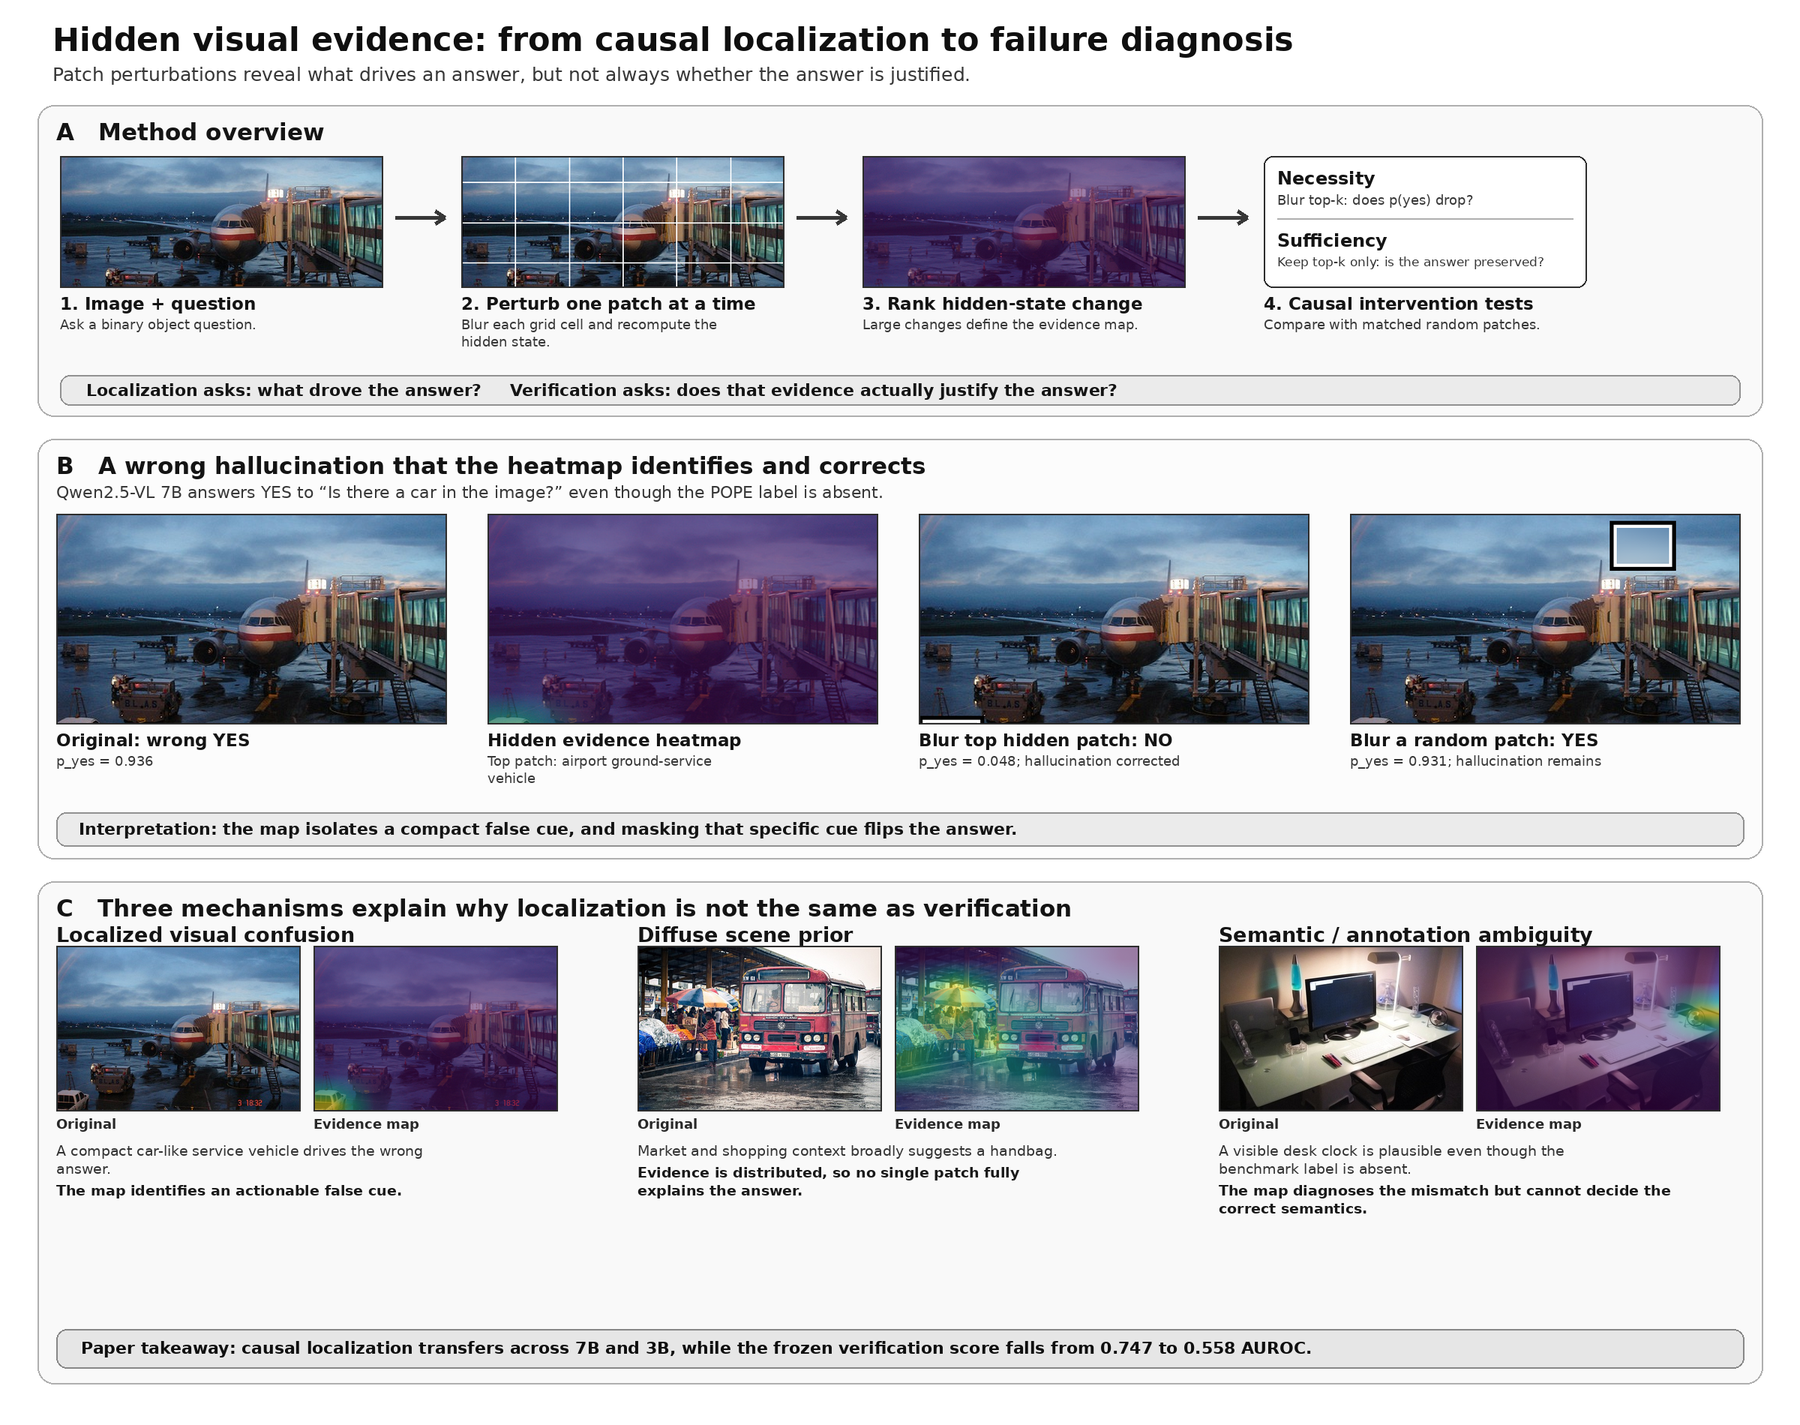
\includegraphics[width=\textwidth]{figures/headline_method_taxonomy_figure_paper.png}
}{
    \fbox{\parbox[c][8cm][c]{0.95\textwidth}{\centering Upload \texttt{headline\_method\_taxonomy\_figure\_paper.png} to the figures folder.}}
}
\caption{Method and failure taxonomy. Patchwise blur interventions rank regions by hidden-state change, followed by matched necessity and sufficiency tests. In the airport example, Qwen 7B hallucinates a car with $p_{\mathrm{yes}}=0.936$ because a compact ground-service vehicle acts as a false cue. Blurring the top hidden patch corrects the answer and lowers $p_{\mathrm{yes}}$ to $0.048$, while a random blur leaves the hallucination nearly unchanged. The remaining examples illustrate diffuse scene priors and semantic or annotation ambiguity, explaining why causal localization does not by itself provide semantic verification.}
\label{fig:taxonomy}
\end{figure*}

\section{Discussion}

The experiments support a precise interpretation of hidden visual evidence. The method identifies regions that strongly influence the representation and answer. This claim is supported by segmentation overlap, full ranking quality, and matched necessity and sufficiency interventions. The method does not determine whether the model's interpretation of those regions is semantically correct.

This distinction explains why attribution based self verification is difficult. In a localized confusion case, the evidence map can be faithful even when the answer is wrong. In a diffuse prior case, no small region may be individually decisive. In an ambiguous benchmark case, the model may be visually reasonable despite a negative label. A single scalar fragility score cannot reliably collapse these mechanisms into correctness.

The result also suggests a more cautious role for visual explanations. They are useful for diagnosing what the model used, auditing false cues, and supporting targeted abstention. They should not be treated as correctness certificates without an additional semantic verification mechanism.

\section{Limitations}

The controlled benchmark evaluates two sizes from one model family. Testing a distinct architecture would strengthen the generalization claim. The $6\times6$ grid is computationally convenient but spatially coarse. Gaussian blur and evidence only images introduce distribution shift, though matched random controls reduce this concern. Verification experiments use yes answers to remove answer identity as a shortcut, but do not cover open ended generation. Finally, the failure taxonomy currently has one provisional reviewer and should receive a second independent annotation pass.

\section{Conclusion}

Hidden state perturbations reliably localize visual evidence that causally drives answers in Qwen2.5 VL 7B and 3B. The selected regions overlap annotated targets, are more necessary than random regions, and are more sufficient than random evidence. Yet a verification score derived from these regions does not transfer across model sizes. The central lesson is that causal attribution and semantic verification are different problems: a model can faithfully reveal what drove its answer without revealing whether the answer is justified.

\bibliographystyle{plainnat}
\bibliography{references}

\end{document}
